L'analisi esplorativa è stata effettuata sull'intero dataset ripulito. 
L'esplorazione dei dati è stata eseguita utilizzando il package R 
\textbf{DataExplorer} e tramite il software \textbf{Power BI}.

Il primo passo è stato visualizzare la distribuzione di colonne con valori 
continui, discreti e mancanti, utilizzando la funzione \texttt{plot\_intro}.

\begin{figure}[htb]
	\centering
	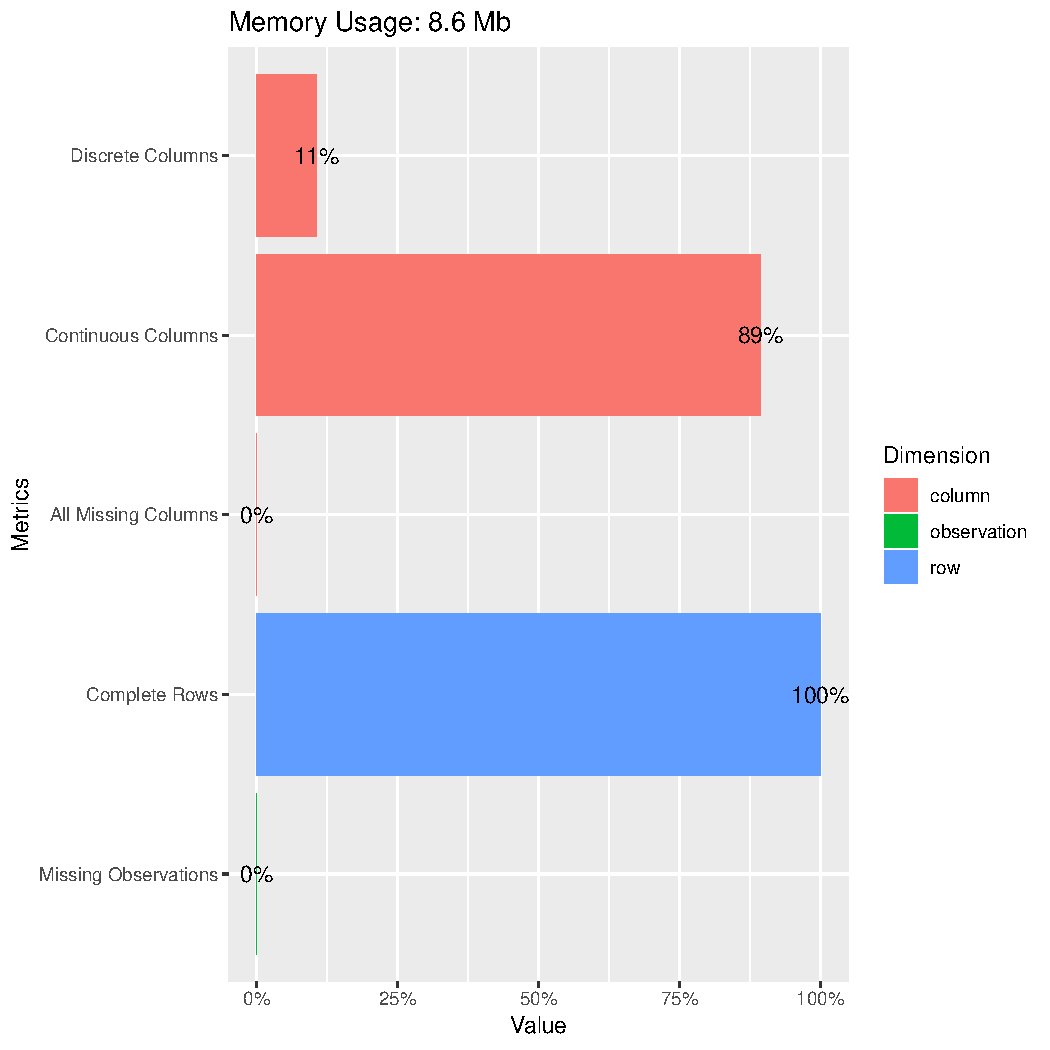
\includegraphics[width=0.4\columnwidth]{images/ml/plot_intro}
	\caption{FIXME}
	\label{fig:plot_intro}
\end{figure}

La maggior parte degli attributi del dataset, precisamente 59, sono di tipo 
continuo, mentre solamente 7 sono di tipo discreto. Di tutto il dataset, 
risulta che, in seguito alla selezione degli attributi alla fine del 
procedimento di integrazione, tutte le righe sono complete al 100\%. 

Per andare nel dettaglio di queste variabili, sono stati generati dei diagrammi 
a barre, con la funzione \texttt{plot\_bar}, per quanto riguarda le variabili 
discrete, e gli istogrammi, tramite la funzione \texttt{plot\_histogram}, delle 
variabili continue.

\begin{figure}[tb]
	\centering
	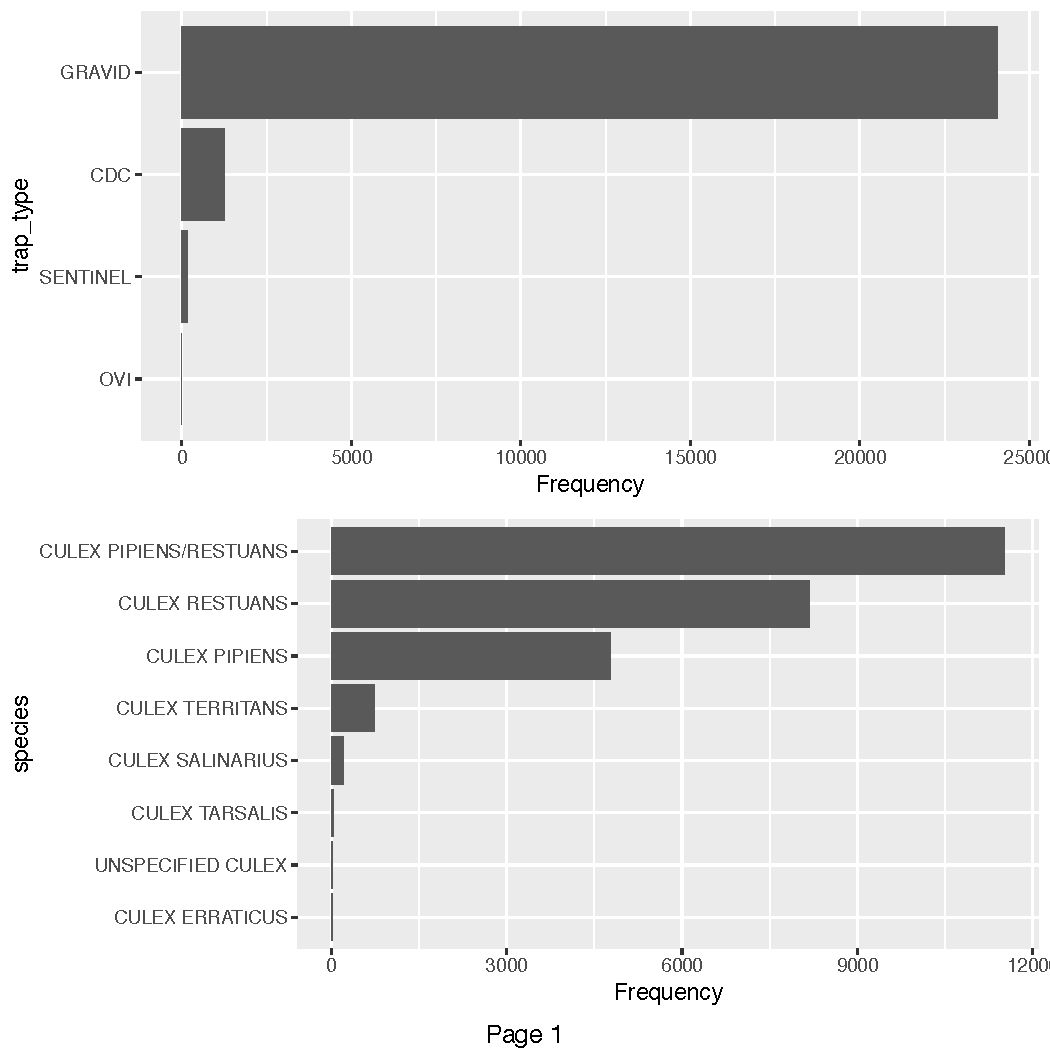
\includegraphics[width=0.57\textwidth]{images/ml/plot_bar1}
	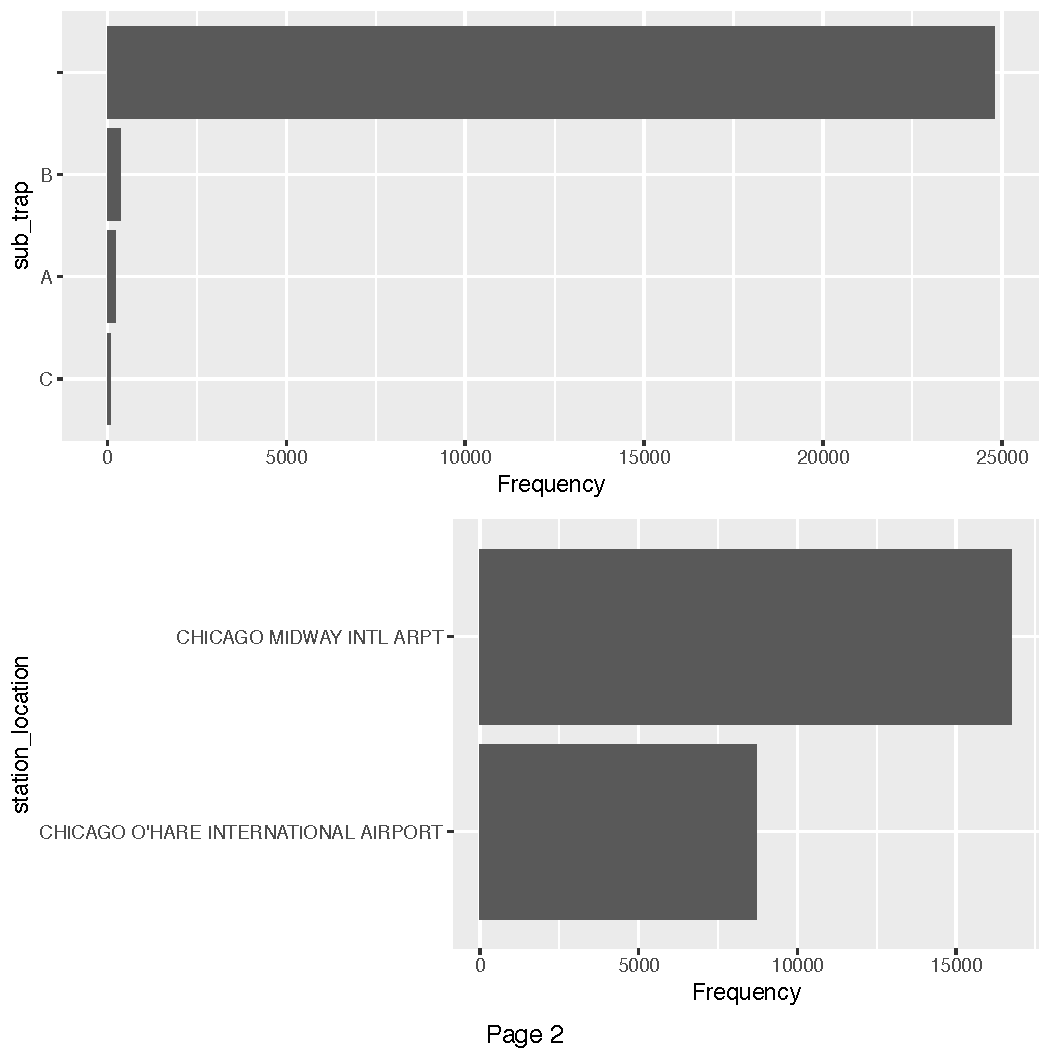
\includegraphics[width=0.3\textwidth]{images/ml/plot_bar2}
	\caption{GRAFICI bar}
	\label{fig:plot_bar}
\end{figure}
Come visibile in figura \ref{fig:plot_bar}, le variabili \texttt{trap\_type} e 
\texttt{result}, che sarebbe il target del nostro modello, hanno una 
distribuzione dei valori non ottimale: quasi la totalità delle trappole sono di 
tipo Gravid, mentre per quanto riguarda \texttt{result}, la maggior parte dei 
test effettuati risultano negativi.
\begin{figure}[H]
	\centering
	\begin{subfigure}[t]{0.49\textwidth}
		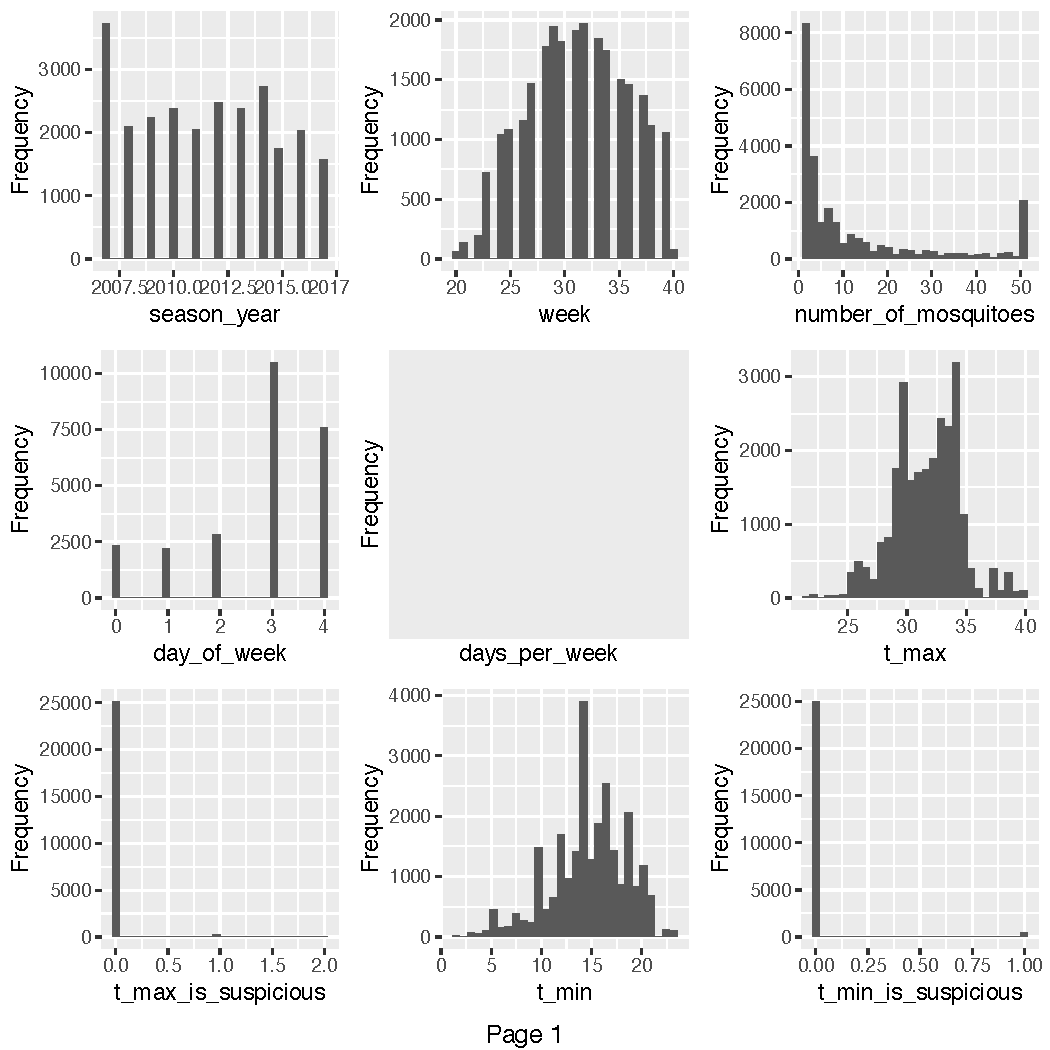
\includegraphics[width=\textwidth]{images/ml/plot_histogram1}
	\end{subfigure}
	\begin{subfigure}[t]{0.49\textwidth}
		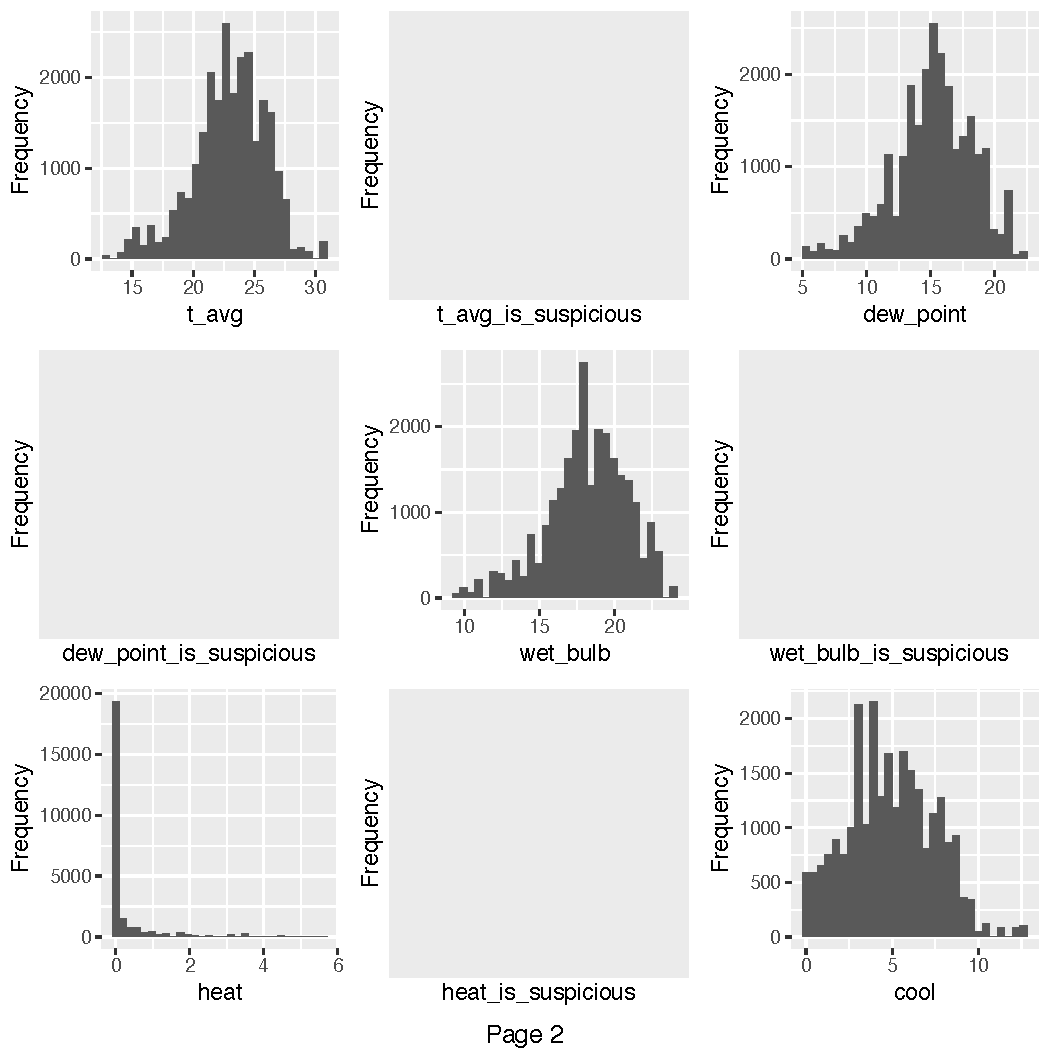
\includegraphics[width=\textwidth]{images/ml/plot_histogram2}
	\end{subfigure}
\end{figure}
\begin{figure}[H]
	\ContinuedFloat 
	\begin{subfigure}[t]{0.49\textwidth}
		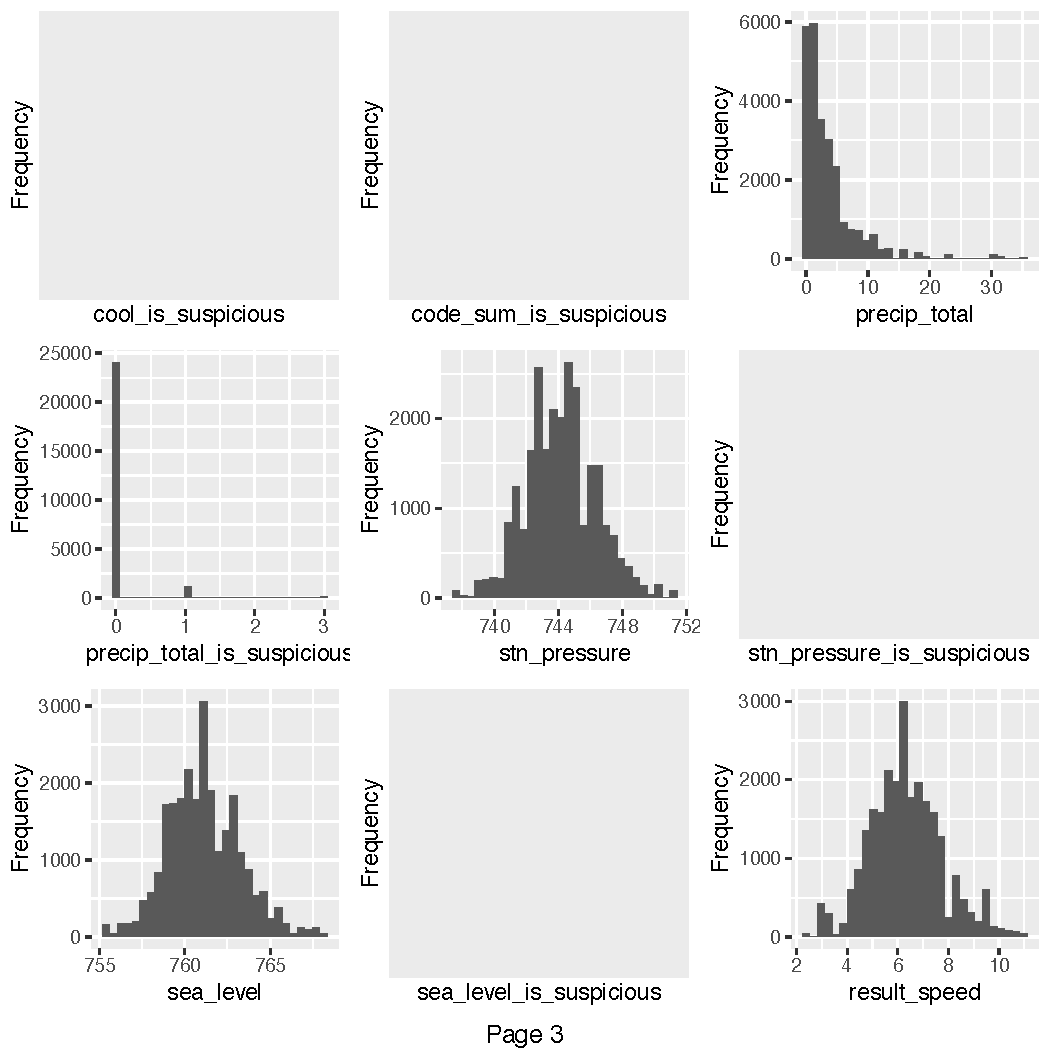
\includegraphics[width=\textwidth]{images/ml/plot_histogram3}
	\end{subfigure}
	\begin{subfigure}[t]{0.49\textwidth}
		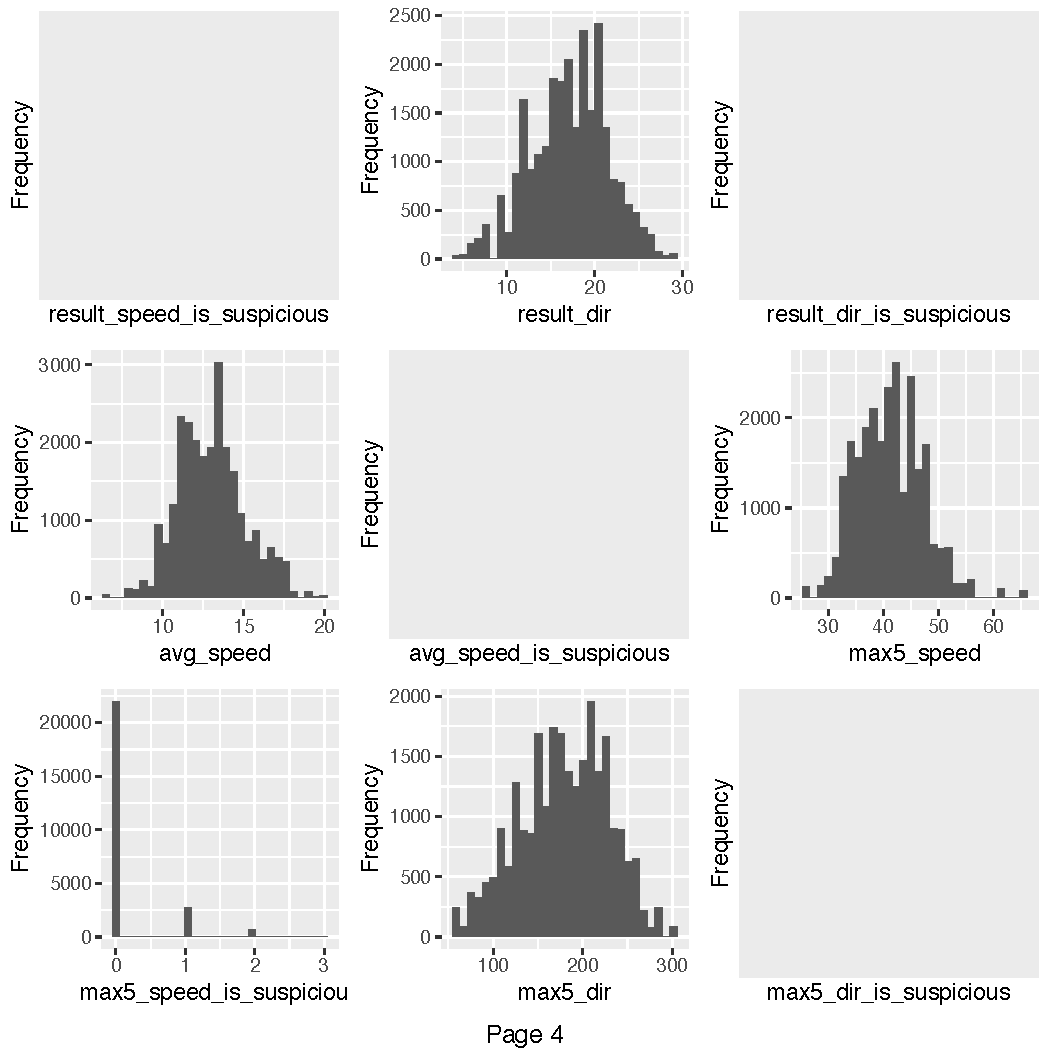
\includegraphics[width=\textwidth]{images/ml/plot_histogram4}
	\end{subfigure}
\end{figure}
\begin{figure}[H]
	\ContinuedFloat 
	\begin{subfigure}[t]{0.49\textwidth}
		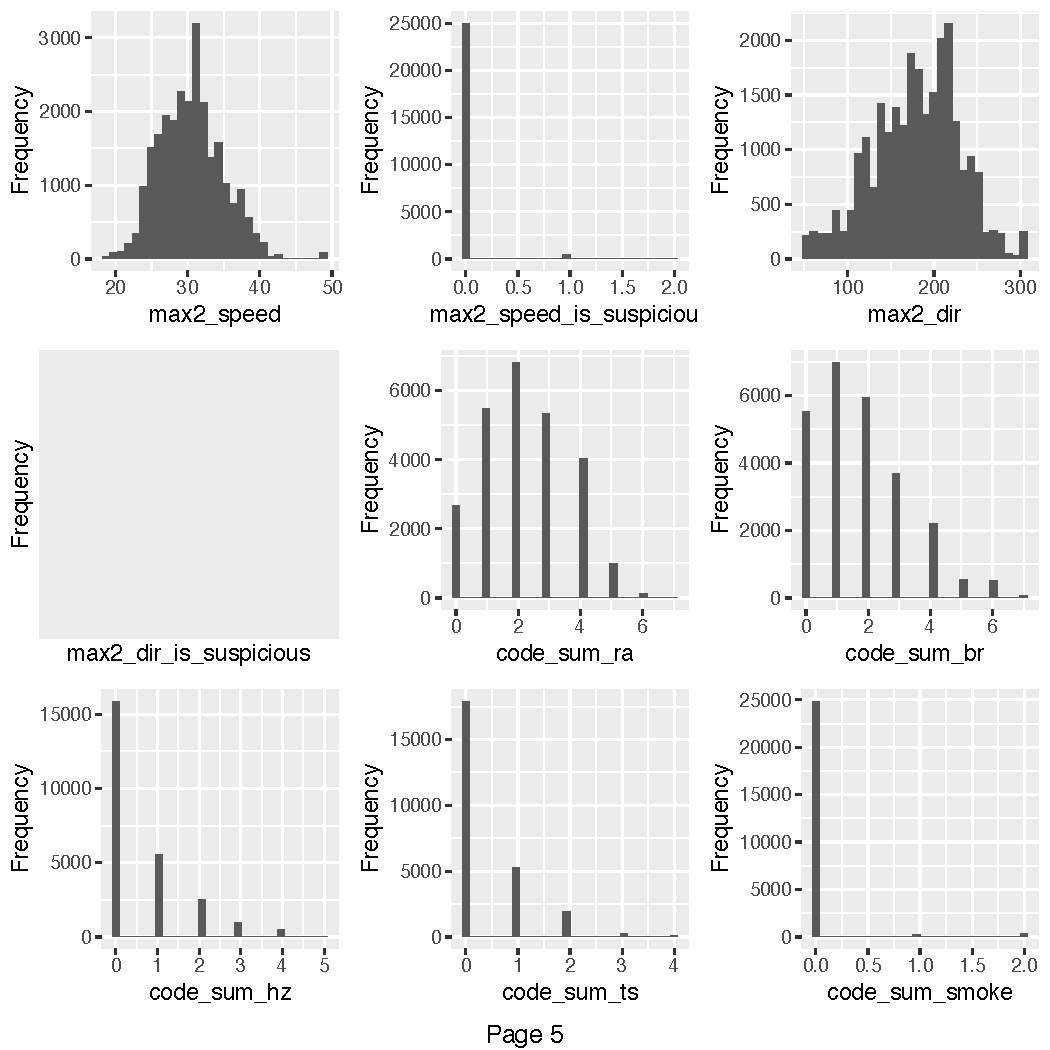
\includegraphics[width=\textwidth]{images/ml/plot_histogram5}
	\end{subfigure}
\caption{GRAFICI istogramma}
\label{fig:plot_histogram}
\end{figure}

La variabile \texttt{number\_of\_mosquitoes} risulta fortemente sbilanciata 
verso valori bassi, ma presenta anche un picco sul valore 50. Questo 
probabilmente deriva del fatto che nel dataset, in caso venga catturato un 
numero di zanzare superiore a 50, questo viene diviso in un altro record con 
gli stessi attributi in modo tale che il numero di zanzare sia limitato a 50.  

Per quanto riguarda l'attributo \texttt{day\_of\_week}, è interessante 
osservare che tutti i test effettuati avvengono nei giorni lavorativi, in 
particolare il giovedì e il venerdì. 


Da questa analisi si evince inoltre che i valori cosiddetti 
 \texttt{suspicious} sono sempre pochi o addirittura non si prestano.

In seguito, per evidenziale eventuali correlazioni tra le variabili del 
dataset, è stata visualizzata una matrice di correlazione, grazie la funzione 
\texttt{plot\_correlation}.

In figura \ref{fig:plot_correlation} viene mostrato il risultato.

\begin{figure}[htb]
	\centering
	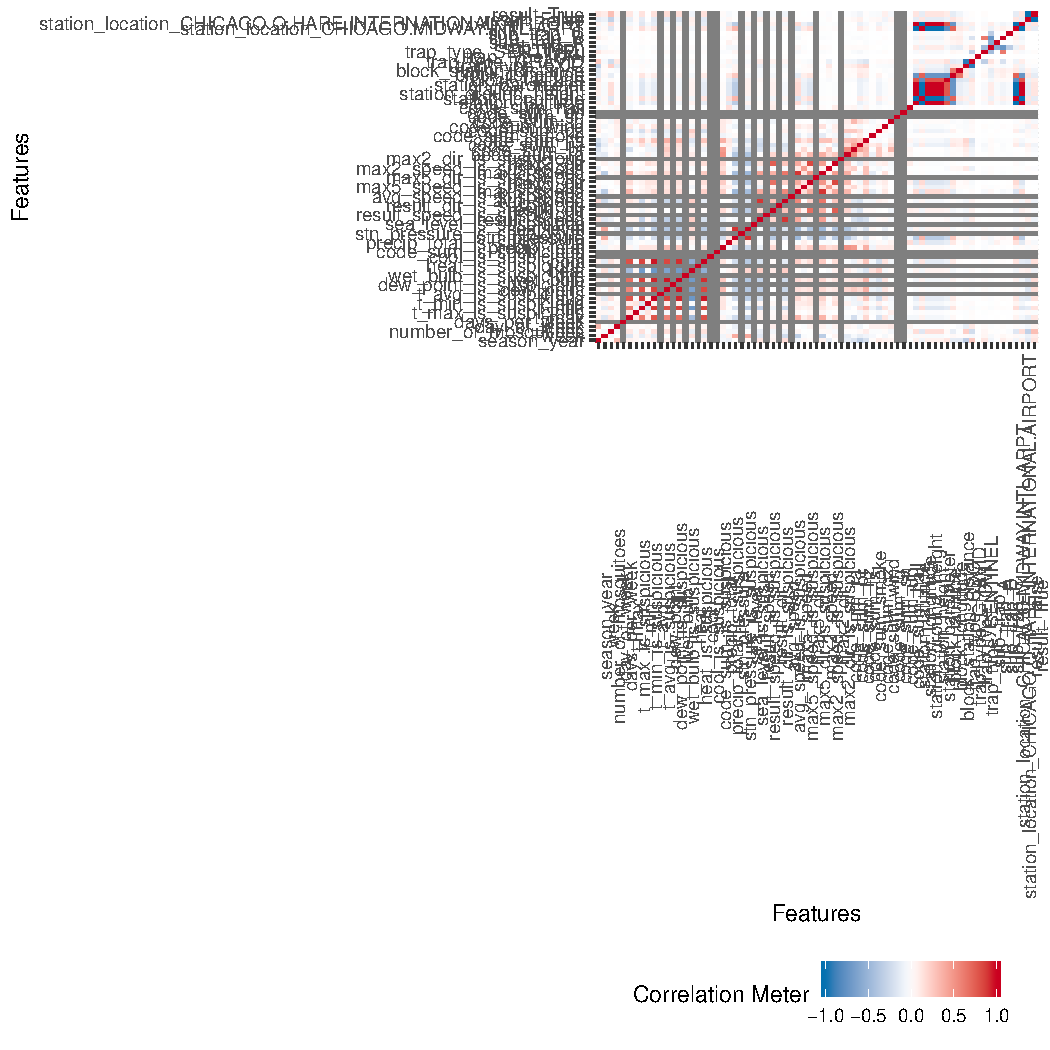
\includegraphics[width=1\columnwidth]{images/ml/plot_correlation}
	\caption{Matrice di correlazione}
	\label{fig:plot_correlation}
\end{figure}

Nell'analisi di questa matrice notiamo la presenza di alcuni cluster di forte 
correlazione, motivati dal fatto che si riferiscono alla due stazioni di 
rilevamento che sono solamente due, e di conseguenza  \textbf{FIXME}.

Alcuni dati riguardanti le feature delle rilevazioni meteo risultano essere più 
correlati di altri, come ad esempio vento e pressione oppure umidità e 
temperatura.

Ponendo l'attenzione sulla variabile \texttt{result}, ovvero il target del 
nostro modello, non sembrerebbe esserci particolari correlazioni con le 
features, eccetto una correlazione poco accentuata con il numero di 
zanzare catturate. Questo è motivato dal fatto che, ipotizzando che prese due 
zanzare, l'evento zanzara infetta o meno sia indipendente, allora è naturale 
che la probabilità che un insieme di zanzare contenga almeno una zanzara 
infetta, cresce linearmente con il numero di zanzare in esso contenute.

Infine è possibile notare un correlazione ancora più lieve tra il target e le 
misure di temperatura. 
